\documentclass{beamer}
\usepackage{amsmath}
\usepackage{amsthm}
\usepackage{graphicx}
\graphicspath{ {./images/}  }

%Information to be included in the title page:
\title{Review: Build a Sporadic Group in Your Basement}
\author{Parker Hyde}
\institute{Georgia State University}
\date{\today}

\begin{document}

\frame{\titlepage}

\begin{frame}
    \frametitle{What is a Group?}
    \begin{itemize}
        \item<2-> \( (G, *) \)
        \item<3->satisfying the properties:
            \begin{enumerate}
                \item closure \( a, b \in G \implies a * b \in G \)
                \item associativity: \(  a * (b * c) = (a * b) * c \ \ \forall a,b,c \in G \) 
                \item existence of identity: \( \exists e \in G \text{ s.t. } a*e = e*a = a \ \forall a \in G \) 
                \item existence of inverses: \( \forall a \in G,  \exists a^{-1} \text { s.t. } a * a^{-1} = a^{-1} * a = e\) 
            \end{enumerate}
    \end{itemize}
    \only<4->{
        \bigbreak
        Examples:
        \( (\mathbb{Z}, +) \) \ 
        %\only<5->{\( S_{n} = (\sigma_n, \circ)\)}
        %\bigbreak
        %\only<6->{ \( \begin{pmatrix}
        %        1 & 2 & 3 & \cdots & n-1 & n \\
        %        2 & 3 & 4 & \cdots &  n  & 1
        %      \end{pmatrix} \in \sigma_n
        %  \) }
    }
\end{frame}
\newtheorem{exmp}{Example}

\begin{frame}
    \frametitle{What is a Sporadic Group?}
    \begin{itemize}
        \item<2-> \( (N,*) \unlhd (G,*) \) 
            \only<3->{ if }
            \begin{enumerate}
                \item<3-> \( N \subset G \), 
                \item<4-> \( N \) is a group under \( * \), and 
                \item<5-> \( g * N = N * g, \ \forall g \in G  \) 
                    \ \ where \( g * N = \{g * n : n \in N \} \)
            \end{enumerate}
        \item<6-> A normal group is a subgroup that partitions it's containing group into 
            a group of \textit{cosets}.
        \item<7-> The result \( \frac{G}{N} = \{g * N : g \in G \}\) is called a \textit{quotient group}.
        %\item<6-> \(\implies \frac{G}{N} = \{ g * N : g \in G \} \) is a group.
        \item<8->
            \begin{example} 
            \end{example}
            \( 5\mathbb{Z} = \{..., -10, -5, 0, 5, 10, ...\} \unlhd \mathbb{Z} \)
        %\item<7-> \( 5\mathbb{Z} \le \mathbb{Z} \) and \( a + 5\mathbb{Z} = 5\mathbb{Z} + a \)
        \item<9-> \( \implies \frac{\mathbb{Z}}{5\mathbb{Z}} 
            = \mathbb{Z}_5 = \{ a + 5\mathbb{Z} : a \in \mathbb{Z} \} 
            = \{ \overline{0}, \overline{1}, \overline{2}, \overline{3}, \overline{4} \}\)
        \item<10-> \( \overline{0} = \{ 0 + 5\mathbb{Z}\} = \{..., -5, 0, 5, 10, 15, ... \}\)\\
         \( \overline{1} = \{ 1 + 5\mathbb{Z}\} = \{..., -4, 1, 6, 11, 16, ...\} \)\\
         \( \overline{2} = \{ 2 + 5\mathbb{Z}\} = \{..., -3, 2, 7, 12, 17, ...\} \)\\
        \item<11-> \( \mathbb{Z}_5 \) is \textit{finite} and \textit{simple}.
    \end{itemize}
    \only<12->{A \textit{sporadic group} is a special kind of finite simple group.}
\end{frame}

\begin{frame}
    \frametitle{Classification of the finite simple groups} 
    \begin{itemize}
        \item<2-> 18 infinite families:
            \begin{enumerate}
                \item<3-> cyclic groups of prime order
                \item<3-> alternating groups \( A_n \), \( n \ge 5 \) 
                \item<4->[3-18.] groups of Lie type
            \end{enumerate}

        \item<5-> 26 Sporadic groups
            \begin{enumerate}
                \item<6-> Mathieu Groups \( M_{11}, M_{12}, M_{22}, M_{23}, M_{24} \)
            \end{enumerate}
    \end{itemize} 
\end{frame}

\begin{frame}
    \frametitle{What is a Sporadic Group?} 
    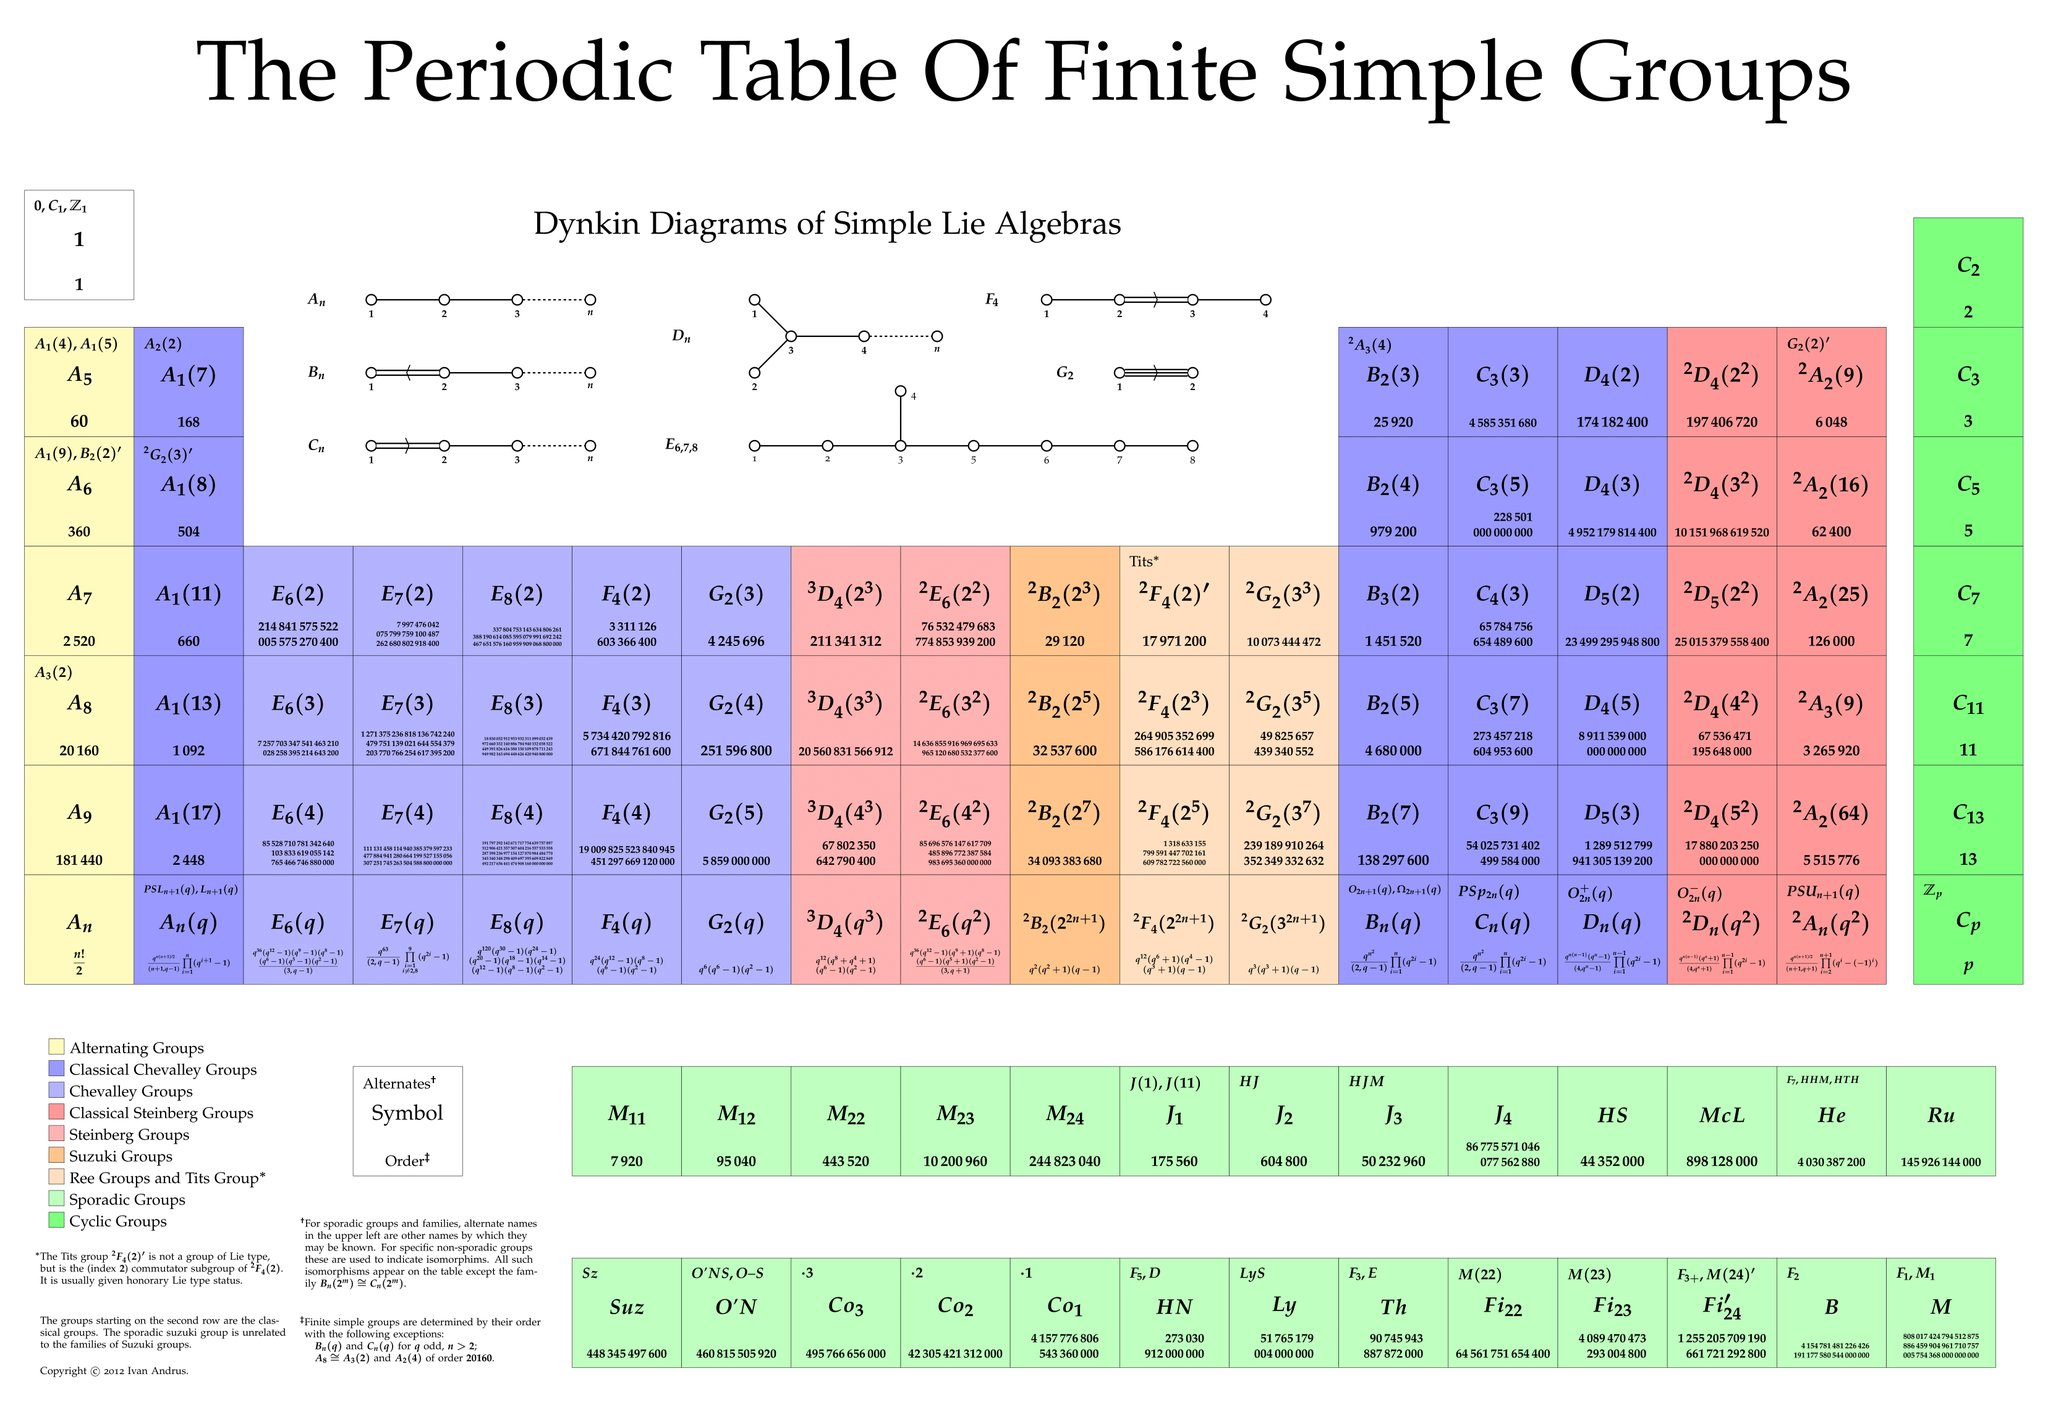
\includegraphics[width=10cm]{periodic}
\end{frame}

\begin{frame}
    \frametitle{What is the Mathieu Group \( M_{24} \)}
\end{frame}



\begin{frame}
    \frametitle{different}
    This is some text in the first frame. This is some text in the first frame. This is some text in the first frame.
\end{frame}
\end{document}
